\section{Concepts}
\label{s:concepts}

Concepts for the design of this device are split into two sub-components:
the grasper (which mechanically attaches the drone to a perch) and the sensor 
(which identifies the location of a suitable perch). 

Each concept below is described with table of components listing estimated cost and 
weight, as well as any preliminary analysis or experimentation performed to identify the 
strengths and weaknesses of the design. The estimated total weight of each concept only
includes the known components of that design, not the material needed for mounting those components
to the drone and to the complementary grasped or sensor design.

\subsection{Grasper Concepts}

\subsubsection{Concept 1}

Shape memory alloys (SMAs) such as Nitinol may be useful for mimicking the grasping of a plant tendril. SMAs transition to
a superelastic state above a threshold temperature. In this state, they are rigid and retain their shape. Below the threshold
temperature, they are malleable. They have the unique property of returning to their "remembered" superelastic when heated back
above the threshold temperature. SMAs have a high strength to weight ratio and due to their malleability can be used for the design of
actuators that mimic organic shapes such as a spiraling plant tendril \cite{baek_dexterous_2023}.
The downside of SMAs in this application is that in order to hold their superelastic form, they must remain heated \cite{wieczorek_smart_2018}.
This would mean the drone must supply current to the grasper to maintain its temperature. This power consumption would negate many of the benefits
of perching, so a method for the grasper to passively hold its position would be needed.


The jamming transition could allow a tendril like actuator to passively hold its position by changing from a flexible form
to a rigid one. With jamming, a volume of particulate matter is held in a flexible container. It is free to be deformed by
external forces until a partial vacuum is applied, after which atmospheric pressure forces the particles to interlock and act
as a solid. This can be accomplished with overlapping sheets or fibers instead of particles as well \cite{fitzgerald_review_2020}.
An example of this is the Universal Gripper \cite{brown_universal_2010}, in which a balloon filled with coffee grounds can
be used to grasp a wide variety of objects. First the balloon is pressed against the object to form to its shape, then a vacuum is
applied and the balloon assumes a rigid form around the object.  


This concept consists of an actuator with 3 SMA wires and a granular core (see Fig. {fig:poses}) cabable 
of transitioning between a flexible and stiff phase via the jamming transition. Jamming will be achieved by 
a syringe-like pump that can draw air out of the core.

The actuator will use SMA wires to actively transition between 3 positions shown in Fig. {fig:poses}:
\begin{itemize}
    \item Home: the tendril is tightly coiled near the drone so as to not obstruct flight.
    \item Extended: The tendril is extended straight up from the drone, for positioning adjacent to a perch.
    \item Coiled: The tendril coils so as to grasp a nearby branch within it.
\end{itemize}
Each transition will be driven by one SMA wire, each wire will be actuated through Joule heating that is activated by the flight controller.



\begin{figure}[H]
    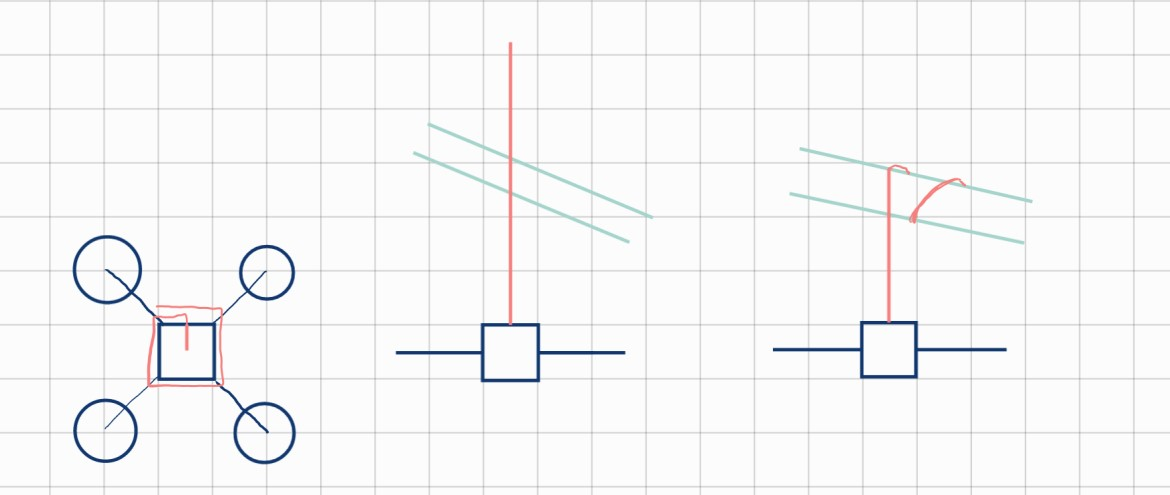
\includegraphics[width=\textwidth]{Poses.jpg}
    \caption{The 3 poses that the actuator (red) will achieve. Home position (left) has the grasper coiled near the drones
    body (blue), for unencumbered flight. In extended position (center) the device reaches straight above the drone to be
    positioned adjacent to a perch (green). While coiled (right), the end of the device grasps around the perch, with some
    length uncoiled so that the drone hangs below the perch.}
    \label{fig:poses}
\end{figure}


A core designed to transition between flexible and solid via the jamming transition (Fig. {fig:crosssec}) will allow the tendril to remain
securely attached when power is removed from the SMA wires. This may be a tube filled with coffee grounds or similar
particles, or it may utilize friction between layers of other material.


\begin{figure}[H]
    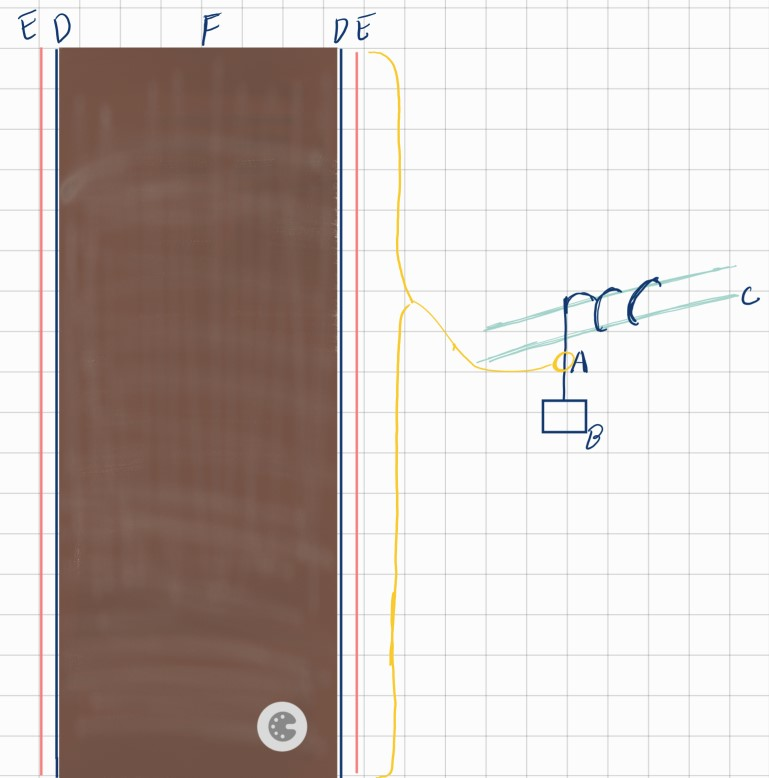
\includegraphics[width=\textwidth]{diagram.jpg}
    \caption{Sketch of the proposed device. The right side shows the device (A)
    attaching a drone (B) to a perch (C). The view on the left shows the flexible core of the device (D),
    two of the 3 SMA wires intended to transition between two positions (E) and the particulate core facilitating
    jamming (F). }
    \label{fig:crosssec}
\end{figure}


The jamming transition will be controlled by a syringe-like linear pump, driven by a servo that is also controlled by the drones flight controller.
Fig. {fig:schematic} shows a simple diagram of the electrical and mechanical components involved in the proposed device.  


\begin{figure}[H]
    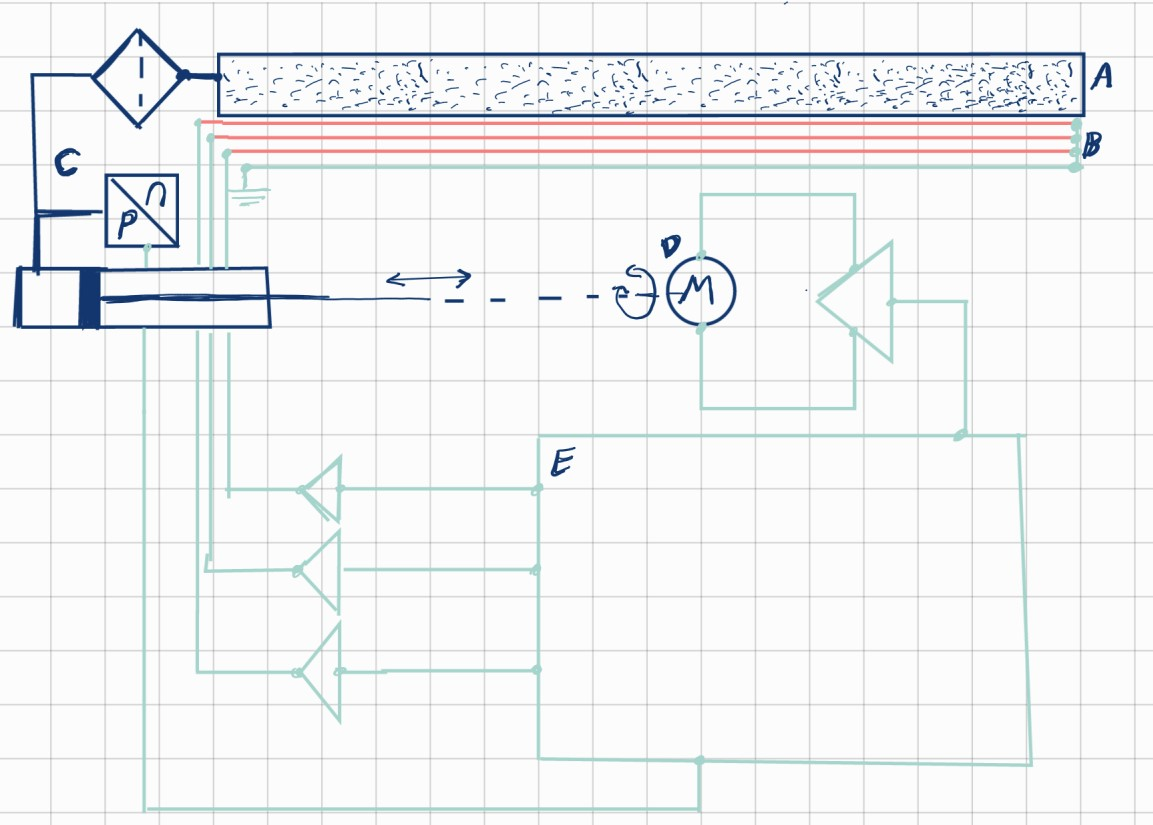
\includegraphics[width=\textwidth]{Schematic.jpg}
    \caption{Block diagram of the proposed device, with mechanical/pneumatic elements in blue, electronics in green,
    and SMA actuators in red. The particulate filled grasper (A) is attached to 3 SMA wires (B), and on one end to
    a filter, pressure sensor, and cylinder/syringe type pump (C). The pump is driven by a motor (D) and suitable
    gear assembly to achieve linear motion. The SMA wires and motor are all driven by the flight control unit (E).}
    \label{fig:schematic}
\end{figure}


To facilitate the jamming transition, a partial vacuum must be produced and maintained within the grasper.
The proposed design will use a servo driven syringe to draw a volume of air from the grasper,
activating the jamming behavior of the coffee grounds within. Two concepts for this mechanism are shown in Fig. {fig:pump}.
They are essentially the same, differing in the type of motor used.


\begin{figure}[H]
    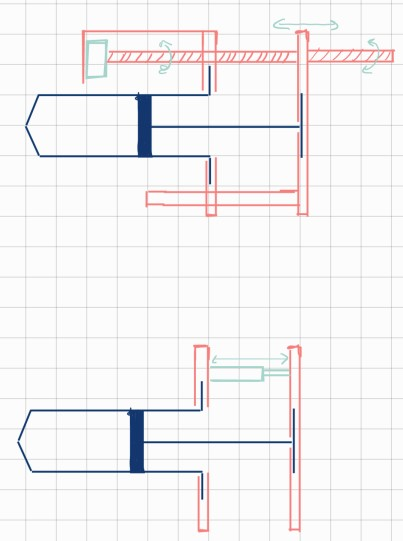
\includegraphics[width=\textwidth]{pump.jpg}
    \caption{Rough depiction of the proposed pump mechanism. Either a rotary motor and screw assembly (top) or
    a pre built linear actuator (bottom) will be used to extend or retract the syringes plunger. The mechanical assembly
    to link the motor and syringe (shown in red) will likely be 3D printed.}
    \label{fig:pump}
\end{figure}


The target pressure within the grasper with jamming activated will be 1/4 atm based on the procedure of Brown et al. \cite{brown_universal_2010}.
Assuming the following points, then  equation \ref{eqn:volume} gives the approximate volume of air to
remove from the grasper core to facilitate jamming.
\begin{itemize}
    \item 34\% porosity of the coffee grounds \cite{oliveros_experimental_2017}.
    \item The bulk of coffee grounds prevent significant volume reduction in
            the grasper core as a result of the pressure change.
    \item Pressure is equal within the grasper and the syringe.
    \item There is no leakage of air through any part of the syringe, grasper, or joining hardware.
\end{itemize}


\begin{eqn}[H]
    \begin{equation}
        \label{eqn:volume}
        V_b = (0.66 V_a) \frac{P_1 - P_2}{P_2}
    \end{equation}
    Where:
    \begin{itemize}
        \item $V_b$ is the volume draw out by the syringe.
        \item $V_a$ is the volume within the grasper, not accounting for the coffee grounds.
        \item $P_1$ is the normal pressure in the grasper, without jamming (1 atm).
        \item $P_2$ is the pressure in the grasper with jamming active (1/4 atm).
    \end{itemize}
\end{eqn}


The grasping device for this proof of concept is planned to be 50cm long. That will provide length to wrap at least on full turn around a perch
up to 15cm in diameter. The grasper core and SMA wires should be as small as possible, to minimize bulk and weight of the device.
Using 50mm of 3mm ID flex tubing for the grasper, $V_a$ is roughly $354 mm^3$.
That gives a volume $V_b$ of roughly $701 mm^3$. A 20mL syringe will provide sufficient volume, with room for error.


To maintain this vacuum, the driving servo must be capable of holding the 3/4 atm
% = 11.02196 psi = 0.075993739093 N / mm2
relative pressure the cylinder will be under. This force is given by equation \ref{eqn:force}.


\begin{eqn}[H]
    \begin{equation}
        \label{eqn:force}
        F = \pi (P_1 - P_2) (\frac{D}{2})^2
    \end{equation}
    Where:
    \begin{itemize}
        \item $F$ is the force sustained by the servo during jamming.
        \item $D$ is the inner diameter of the syringe.
        \item $P_1$ is the normal pressure in the grasper, without jamming (1 atm).
        \item $P_2$ is the pressure in the grasper with jamming active (1/4 atm).
    \end{itemize}
\end{eqn}


With a syringe having an inner diameter of 2cm, this gives a required force of 23.87 N or 5.37 lbs.
% 3/4 atm = 7.5994 N/cm2

\paragraph{Budget}


The estimated cost for components needed for this thesis is shown in table \ref{tab:grasper}. The design will utilize materials and tools available for student projects
in engineering facilities as much as possible, for example 3D printing or machining mechanical components, as well as other materials that are freely available, such as
coffee grounds and 20 mL syringes (which the author has left over from other projects).


The budget includes an estimated 7\% sales tax on all materials, as well as an additional 20\% of the total estimate
to account for any spare or replacement parts that are needed during development and testing.


\begin{table}[ht]
    \centering
    \caption{Estimated budget for the grasper design.}
    \label{tab:grasper}


    \begin{spreadtab}{{tabular}{|c|c|c|c||c|}}
        \hline
        @Item                       & @Supplier                                                                                                         & @Unit Cost (USD) & @Quantity & @Total Cost (USD) \\
        \hline
        @SMA Wire                   & @\href{https://www.kelloggsresearchlabs.com/product/round-wire/}{Kelloggs Research Labs}                          & 15.99 & 1 & [-1,0] * [-2,0] tag(start) \\
        @Kellogs Shipping           & @-                                                                                                                &  4.99 & 1 & [-1,0] * [-2,0] \\
        @Servo                      & @\href{https://www.digikey.com/en/products/detail/actuonix-motion-devices-inc/L16-50-150-6-R/11689514}{Digikey}   & 90.00 & 1 & [-1,0] * [-2,0] \\
        @Digikey Shipping           & @-                                                                                                                & 14.99 & 1 & [-1,0] * [-2,0] \\
        @Pneumatic Tube             & @\href{https://www.adafruit.com/product/4661}{Adafruit}                                                           &  2.50 & 1 & [-1,0] * [-2,0] \\
        @Amplifiers                 & @\href{https://www.adafruit.com/product/355}{Adafruit}                                                            &  2.25 & 3 & [-1,0] * [-2,0] \\
        @Arduino                    & @\href{https://www.adafruit.com/product/2378}{Adafruit}                                                           & 11.95 & 1 & [-1,0] * [-2,0] \\
        @FTDI Programmer            & @\href{https://www.adafruit.com/product/70}{Adafruit}                                                             & 19.95 & 1 & [-1,0] * [-2,0] \\
        @Pressure Sensor            & @\href{https://www.adafruit.com/product/3965}{Adafruit}                                                           & 29.95 & 1 & [-1,0] * [-2,0] \\
        @Limit Switches             & @\href{https://www.adafruit.com/product/818}{Adafruit}                                                            &  1.50 & 2 & [-1,0] * [-2,0] \\
        @Adafruit Shipping          & @-                                                                                                                &  5.08 & 1 & [-1,0] * [-2,0] \\
        @Syringe                    & @-                                                                                                                &     0 & 1 & [-1,0] * [-2,0] \\
        @Coffee Grounds             & @-                                                                                                                &     0 & 1 & [-1,0] * [-2,0] \\
        @PCB Material               & @\href{https://www.mcmaster.com/8521K873}{McMaster Carr}                                                          & 12.45 & 1 & [-1,0] * [-2,0] \\
        @McMaster Carr Shipping     & @-                                                                                                                & 10.02 & 1 & [-1,0] * [-2,0] \\
        @Mechanical Materials and Fabrication & @-                                                                                                      &     0 & 1 & [-1,0] * [-2,0] tag(pretax)\\
        @Tax                        & @- & sum(cell(start):cell(pretax)) * 0.07 & 1 & [-1,0] * [-2,0] tag(posttax) \\
        @Misc. Spares               & @- & sum(cell(start):cell(posttax)) * 0.2 & 1 & [-1,0] * [-2,0] tag(end) \\
        \hline
        \multicolumn{4}{|c||}{@Total} & sum(cell(start):cell(end)) \\
        \hline
    \end{spreadtab}
\end{table}


\paragraph{Evaluation}

Initial testing of this concept was done silicone tubing with inner diameter of 3mm and outer diameter of 5mm.
The tube was filled with coffee grounds. One end was plugged with a portion of a wooden skewer and secured with a zip tie,
and the other end secured with a zip tie to a 20mL syringe. 

Extending the syringe to its maximum volume (applying maximum vacuum) showed little change in the stiffness of the design.
This is possibly due to the thickness of the silicone tube. The actuator designed by Brown et al. \cite{brown_universal_2010} 
used a balloon, which is thinner and more flexible allowing the coffee grounds inside to bear the load of the vacuum. 
The tube in this test was thicker and stiffer, so less of the pressure was transferred to the coffee grounds inside,
preventing a change in stiffness. 

A second attempt with a thinner tube (a balloon, the long type used to make balloon animals) showed little improvement. 
There was no noticeable change in the stiffness of the device. This may indicate that the estimates for how much pressure is needed
or the volume of air withdrawn required to create this pressure are too low. Making the device capable of withdrawing more air would likely
result in too large and heavy of a final design. It is also possible that the failure of this concept is due to the small diameter of the
grasper not providing enough strength to resist deformation. Fixing this would also require the device to be larger and heavier.




\subsubsection{Concept 2}

This concept aims to overcome the problems with the jamming transition encountered by concept 1.
SMA wires are still used for actuation, however rather than a variable stiffness mechanism a mechanical latch will
be used to secure SMA wires around the perch.

This concept can be imagined somewhat like a padlock, roughly illustrated in Fig. \ref{fig:lock}. 
A set of 3 SMA wires will still be used to move between 
home, extended, and latched position. At the end of the wires will be a loop through
which a solenoid, servo, or similar latching mechanism can slide.

\begin{figure}[H]
    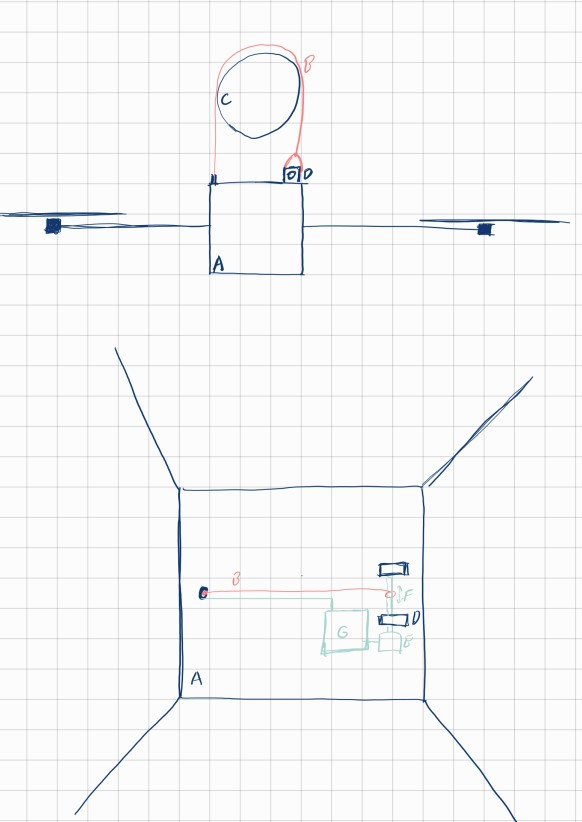
\includegraphics[width=\textwidth]{Lock.jpg}
    \caption{Rough depiction of the lock-like grasping mechanism. Shown is a side profile (top) and a top profile (bottom) 
    of a drone body (A). The SMA wire grasper (B) is shown with a loop at one end, to attach to the latching mechanism (D,F).
    The latch would be driven into place by a small servo (E), controlled from the same unit driving the SMA amplifiers (G).}
    \label{fig:lock}
\end{figure}


\paragraph{Budget}

\begin{table}[ht]
    \centering
    \caption{Estimated budget for the lock design.}
    \label{tab:lock}


    \begin{spreadtab}{{tabular}{|c|c|c|c||c|}}
        \hline
        @Item                       & @Supplier                                                                                                         & @Unit Cost (USD) & @Quantity & @Total Cost (USD) \\
        \hline
        @SMA Wire                   & @\href{https://www.kelloggsresearchlabs.com/product/round-wire/}{Kelloggs Research Labs}                          & 15.99 & 1 & [-1,0] * [-2,0] tag(start) \\
        @Kellogs Shipping           & @-                                                                                                                &  4.99 & 1 & [-1,0] * [-2,0] \\
        @Servo                      & @\href{https://www.digikey.com/en/products/detail/actuonix-motion-devices-inc/L16-50-150-6-R/11689514}{Digikey}   & 90.00 & 1 & [-1,0] * [-2,0] \\
        @Digikey Shipping           & @-                                                                                                                & 14.99 & 1 & [-1,0] * [-2,0] \\
        @Amplifiers                 & @\href{https://www.adafruit.com/product/355}{Adafruit}                                                            &  2.25 & 3 & [-1,0] * [-2,0] \\
        @Arduino                    & @\href{https://www.adafruit.com/product/2378}{Adafruit}                                                           & 11.95 & 1 & [-1,0] * [-2,0] \\
        @FTDI Programmer            & @\href{https://www.adafruit.com/product/70}{Adafruit}                                                             & 19.95 & 1 & [-1,0] * [-2,0] \\
        @Adafruit Shipping          & @-                                                                                                                &  5.08 & 1 & [-1,0] * [-2,0] \\
        @PCB Material               & @\href{https://www.mcmaster.com/8521K873}{McMaster Carr}                                                          & 12.45 & 1 & [-1,0] * [-2,0] \\
        @McMaster Carr Shipping     & @-                                                                                                                & 10.02 & 1 & [-1,0] * [-2,0] \\
        @Mechanical Materials and Fabrication & @-                                                                                                      &     0 & 1 & [-1,0] * [-2,0] tag(pretax)\\
        @Tax                        & @- & sum(cell(start):cell(pretax)) * 0.07 & 1 & [-1,0] * [-2,0] tag(posttax) \\
        @Misc. Spares               & @- & sum(cell(start):cell(posttax)) * 0.2 & 1 & [-1,0] * [-2,0] tag(end) \\
        \hline
        \multicolumn{4}{|c||}{@Total} & sum(cell(start):cell(end)) \\
        \hline
    \end{spreadtab}
\end{table}


\paragraph{Evaluation}

This design has the benefit of being simpler than concept 1, and could possible be made significantly smaller and lighter.

One immediately apparent weakness of this design is that it will not fit to the form of its perch as the coiling, tendril-like 
concept will. This could reduce friction that prevents the drone from swinging on its perch, or sliding back and forth. 
This may possibly be minimized by adding high friction material or spikes to the SMA actuator.


\subsubsection{Concept 3} 

This concept attempts to alleviate the concerns with concept 2, regarding being unable to hold a
stable orientation on a perch. This is done with the addition of microspine devices similar to those used by
Nguyen et al. in their grapple device \cite{nguyen_passively_2019}. 

This concept would use the same design as concept 2, however the loop portion that wraps around a perch would
have the addition of microspines that help grip the perch and stabilize the position and orientation of the drone.


\paragraph{Budget}

\begin{table}[ht]
    \centering
    \caption{Estimated budget for the lock design with microspines.}
    \label{tab:lock_spines}


    \begin{spreadtab}{{tabular}{|c|c|c|c||c|}}
        \hline
        @Item                       & @Supplier                                                                                                         & @Unit Cost (USD) & @Quantity & @Total Cost (USD) \\
        \hline
        @SMA Wire                   & @\href{https://www.kelloggsresearchlabs.com/product/round-wire/}{Kelloggs Research Labs}                          & 15.99 & 1 & [-1,0] * [-2,0] tag(start) \\
        @Kellogs Shipping           & @-                                                                                                                &  4.99 & 1 & [-1,0] * [-2,0] \\
        @Servo                      & @\href{https://www.digikey.com/en/products/detail/actuonix-motion-devices-inc/L16-50-150-6-R/11689514}{Digikey}   & 90.00 & 1 & [-1,0] * [-2,0] \\
        @Digikey Shipping           & @-                                                                                                                & 14.99 & 1 & [-1,0] * [-2,0] \\
        @Amplifiers                 & @\href{https://www.adafruit.com/product/355}{Adafruit}                                                            &  2.25 & 3 & [-1,0] * [-2,0] \\
        @Arduino                    & @\href{https://www.adafruit.com/product/2378}{Adafruit}                                                           & 11.95 & 1 & [-1,0] * [-2,0] \\
        @FTDI Programmer            & @\href{https://www.adafruit.com/product/70}{Adafruit}                                                             & 19.95 & 1 & [-1,0] * [-2,0] \\
        @Adafruit Shipping          & @-                                                                                                                &  5.08 & 1 & [-1,0] * [-2,0] \\
        @PCB Material               & @\href{https://www.mcmaster.com/8521K873}{McMaster Carr}                                                          & 12.45 & 1 & [-1,0] * [-2,0] \\
        @McMaster Carr Shipping     & @-                                                                                                                & 10.02 & 1 & [-1,0] * [-2,0] \\
        @Mechanical Materials and Fabrication & @-                                                                                                      &     0 & 1 & [-1,0] * [-2,0] tag(pretax)\\
        @Tax                        & @- & sum(cell(start):cell(pretax)) * 0.07 & 1 & [-1,0] * [-2,0] tag(posttax) \\
        @Misc. Spares               & @- & sum(cell(start):cell(posttax)) * 0.2 & 1 & [-1,0] * [-2,0] tag(end) \\
        \hline
        \multicolumn{4}{|c||}{@Total} & sum(cell(start):cell(end)) \\
        \hline
    \end{spreadtab}
\end{table}

\paragraph{Evaluation}

The downside of the microspine additions is that they would add weight and bulk to the SMA wire portion of the device.
This would impact flight time and stability, and possibly destabilize the drone during perching when the wires are extended.
They would also be designed to perch on certain materials, such as wood, better than others. On smooth surfaces they may
provide no benefit. 


\subsubsection{Concept 4} 

This concept is nearly identical to concept 3, except that it replaces the SMA actuation with 
a cable actuated curling grasper that moves a loop into a locked position. The main motivation for this 
concept is that the authors lack of familiarity with SMAs poses a risk to the timeline of this thesis.


%% TODO: Update This
\paragraph{Budget}

\begin{table}[ht]
    \centering
    \caption{Estimated budget for the lock design with microspines.}
    \label{tab:lock_flex}


    \begin{spreadtab}{{tabular}{|c|c|c|c||c|}}
        \hline
        @Item                       & @Supplier                                                                                                         & @Unit Cost (USD) & @Quantity & @Total Cost (USD) \\
        \hline
        @SMA Wire                   & @\href{https://www.kelloggsresearchlabs.com/product/round-wire/}{Kelloggs Research Labs}                          & 15.99 & 1 & [-1,0] * [-2,0] tag(start) \\
        @Kellogs Shipping           & @-                                                                                                                &  4.99 & 1 & [-1,0] * [-2,0] \\
        @Servo                      & @\href{https://www.digikey.com/en/products/detail/actuonix-motion-devices-inc/L16-50-150-6-R/11689514}{Digikey}   & 90.00 & 1 & [-1,0] * [-2,0] \\
        @Digikey Shipping           & @-                                                                                                                & 14.99 & 1 & [-1,0] * [-2,0] \\
        @Amplifiers                 & @\href{https://www.adafruit.com/product/355}{Adafruit}                                                            &  2.25 & 3 & [-1,0] * [-2,0] \\
        @Arduino                    & @\href{https://www.adafruit.com/product/2378}{Adafruit}                                                           & 11.95 & 1 & [-1,0] * [-2,0] \\
        @FTDI Programmer            & @\href{https://www.adafruit.com/product/70}{Adafruit}                                                             & 19.95 & 1 & [-1,0] * [-2,0] \\
        @Adafruit Shipping          & @-                                                                                                                &  5.08 & 1 & [-1,0] * [-2,0] \\
        @PCB Material               & @\href{https://www.mcmaster.com/8521K873}{McMaster Carr}                                                          & 12.45 & 1 & [-1,0] * [-2,0] \\
        @McMaster Carr Shipping     & @-                                                                                                                & 10.02 & 1 & [-1,0] * [-2,0] \\
        @Mechanical Materials and Fabrication & @-                                                                                                      &     0 & 1 & [-1,0] * [-2,0] tag(pretax)\\
        @Tax                        & @- & sum(cell(start):cell(pretax)) * 0.07 & 1 & [-1,0] * [-2,0] tag(posttax) \\
        @Misc. Spares               & @- & sum(cell(start):cell(posttax)) * 0.2 & 1 & [-1,0] * [-2,0] tag(end) \\
        \hline
        \multicolumn{4}{|c||}{@Total} & sum(cell(start):cell(end)) \\
        \hline
    \end{spreadtab}
\end{table}

\paragraph{Evaluation}



\subsubsection{Concept 5} 

This concept uses a cable actuated grasper like concept 4, however this concept would coil similar 
to the grasping behavior of a plant tendril as described by \cite{klimm_force_2023}. This could produce
tighter grasping of objects of varying size and shape than concept 3 could, however it would require some amount of
continuous power draw to maintain grasping force.


%% TODO: Update This
\paragraph{Budget}

\begin{table}[ht]
    \centering
    \caption{Estimated budget for the lock design with microspines.}
    \label{tab:cable_coil}


    \begin{spreadtab}{{tabular}{|c|c|c|c||c|}}
        \hline
        @Item                       & @Supplier                                                                                                         & @Unit Cost (USD) & @Quantity & @Total Cost (USD) \\
        \hline
        @SMA Wire                   & @\href{https://www.kelloggsresearchlabs.com/product/round-wire/}{Kelloggs Research Labs}                          & 15.99 & 1 & [-1,0] * [-2,0] tag(start) \\
        @Kellogs Shipping           & @-                                                                                                                &  4.99 & 1 & [-1,0] * [-2,0] \\
        @Servo                      & @\href{https://www.digikey.com/en/products/detail/actuonix-motion-devices-inc/L16-50-150-6-R/11689514}{Digikey}   & 90.00 & 1 & [-1,0] * [-2,0] \\
        @Digikey Shipping           & @-                                                                                                                & 14.99 & 1 & [-1,0] * [-2,0] \\
        @Amplifiers                 & @\href{https://www.adafruit.com/product/355}{Adafruit}                                                            &  2.25 & 3 & [-1,0] * [-2,0] \\
        @Arduino                    & @\href{https://www.adafruit.com/product/2378}{Adafruit}                                                           & 11.95 & 1 & [-1,0] * [-2,0] \\
        @FTDI Programmer            & @\href{https://www.adafruit.com/product/70}{Adafruit}                                                             & 19.95 & 1 & [-1,0] * [-2,0] \\
        @Adafruit Shipping          & @-                                                                                                                &  5.08 & 1 & [-1,0] * [-2,0] \\
        @PCB Material               & @\href{https://www.mcmaster.com/8521K873}{McMaster Carr}                                                          & 12.45 & 1 & [-1,0] * [-2,0] \\
        @McMaster Carr Shipping     & @-                                                                                                                & 10.02 & 1 & [-1,0] * [-2,0] \\
        @Mechanical Materials and Fabrication & @-                                                                                                      &     0 & 1 & [-1,0] * [-2,0] tag(pretax)\\
        @Tax                        & @- & sum(cell(start):cell(pretax)) * 0.07 & 1 & [-1,0] * [-2,0] tag(posttax) \\
        @Misc. Spares               & @- & sum(cell(start):cell(posttax)) * 0.2 & 1 & [-1,0] * [-2,0] tag(end) \\
        \hline
        \multicolumn{4}{|c||}{@Total} & sum(cell(start):cell(end)) \\
        \hline
    \end{spreadtab}
\end{table}

\paragraph{Evaluation}


\subsection{Sensing Concepts}

\subsubsection{Concept 1}

The first concept is the use of a stereo vision camera to detect a suitable object to perch from.
This appreach has been established in existing literature, such as the perching mechanisms developed by
Kominami et al. \cite{kominami_detection_2023} and von Frankenberg et al. \cite{von_frankenberg_detection_2020}.

Dual cameras would be used to calculate a depth map, from which the location and orientation of a perchable object, like 
a tree branch or power line, can then be detected. 

A proof of concept image processing pipeline for this method was developed and tested in Python.
It is based on the method proposed by Kominami et al., in which a Hough transform detects the two
sides of a possible perch, and the depth profile along a path perpendicular to the two lines is 
used to verify that the detected object is a suitable perch \cite{kominami_detection_2023}.
Modifications to the exact detection method and criteria are made to address the difference 
in perch types between Kominami et al. and this work; while Kominami at al. are focusing 
on detecting thin vertical boards, this mechanism needs to itentify cylindrical shapes.

The steps in the pipeline proposed are as follows:

\begin{enumerate}
    \item Stereo image aquisition:
        Images from two cameras are aquired, rectified, and processed to produce a disparity image.
    \item The disparity image is projected to a point cloud in the left cameras cordinate frame,
        then converted to a depth image.
    \item Missing data in the depth image is inpainted using the Fast Marching Method developed by
        Telea \cite{telea_image_2004}.
    \item The depth image is filtered using guided filtering \cite{he_guided_2013}, 
        with the left cameras refified grayscale image as a guide. This is intended to
        remove noise while preserving sharp details of object borders.
    \item A Canny edge detector is applied to the grayscale image of the left camera.
    \item A probabilistic Hough transform is applied to identify line segments in the image.
    \item Parallel pairs are identified from the set of line segments.
    \item For each parallel pair, a perpendicular line is found and the depth profile along 
        that line is sampled.
\end{enumerate}


\paragraph{Budget}

\begin{table}[ht]
    \centering
    \caption{Estimated budget for the stereo camera sensing design.}
    \label{tab:stereo}


    \begin{spreadtab}{{tabular}{|c|c|c|c||c|}}
        \hline
        @Item                       & @Supplier                                                                                                         & @Unit Cost (USD) & @Quantity & @Total Cost (USD) \\
        \hline
        @SMA Wire                   & @\href{https://www.kelloggsresearchlabs.com/product/round-wire/}{Kelloggs Research Labs}                          & 15.99 & 1 & [-1,0] * [-2,0] tag(start) \\
        @Mechanical Materials and Fabrication & @-                                                                                                      &     0 & 1 & [-1,0] * [-2,0] tag(pretax)\\
        @Tax                        & @- & sum(cell(start):cell(pretax)) * 0.07 & 1 & [-1,0] * [-2,0] tag(posttax) \\
        @Misc. Spares               & @- & sum(cell(start):cell(posttax)) * 0.2 & 1 & [-1,0] * [-2,0] tag(end) \\
        \hline
        \multicolumn{4}{|c||}{@Total} & sum(cell(start):cell(end)) \\
        \hline
    \end{spreadtab}
\end{table}


\paragraph{Evaluation}

The main downside of this method is that it is the highest cost and weight of all the options, due to 
the requirement of two cameras. Aquiring quality depth images with low processing time is another challenge.
The disparity maps produced by block matching are noisy and have many patches of missing data. Inpainting
and guided filtering help with this, but there remain a large number of artifacts in the depth data
that interfere with identifying suitable objects for perching.

Figure \ref{fig:c1:depth_profiles} shows images from the proof of concept pipeline, obtained from 
processing figure \ref{fig:c1:testimg}. All image processing functions used are implemented by OpenCV.

\begin{figure}[H]
    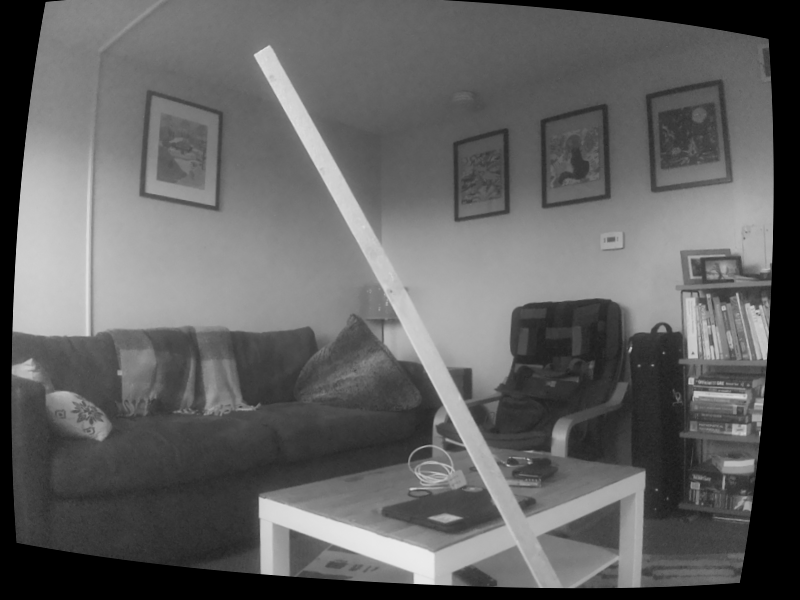
\includegraphics[width=0.5\textwidth]{sections/sensor_concepts/left.png}
    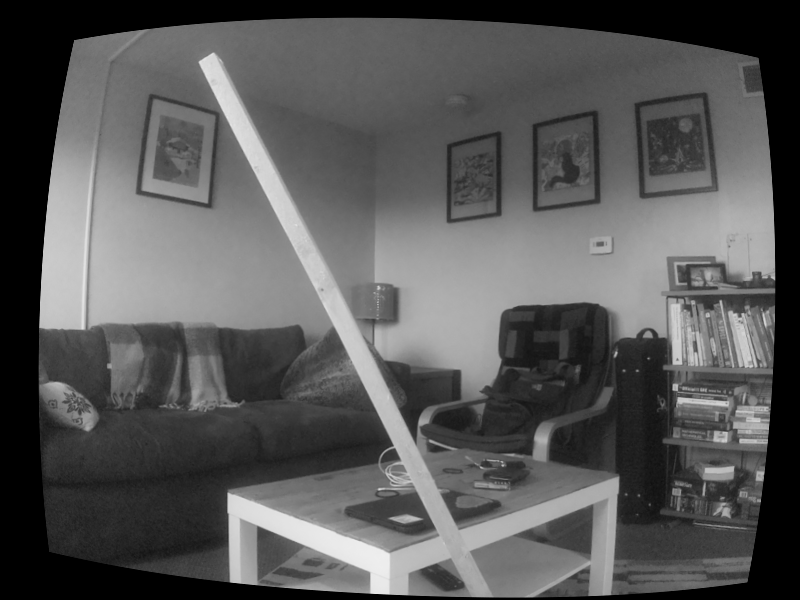
\includegraphics[width=0.5\textwidth]{sections/sensor_concepts/right.png}
    \caption{Captures from left and right cameras used as input in this proof of concept.
    In the center of the frame is a rectangular wooden plank, used as a target perch to detect.
    }
    \label{fig:c1:testimg}
\end{figure}

\begin{figure}[H]
    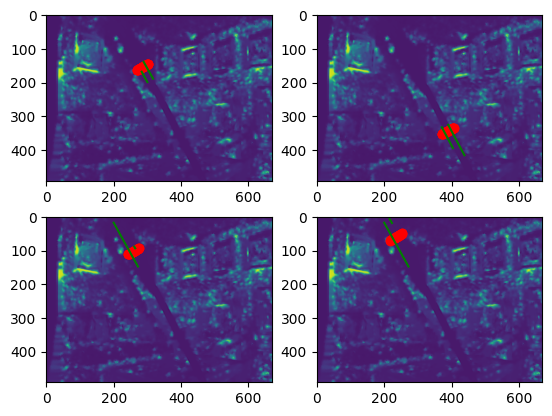
\includegraphics[width=0.5\textwidth]{sections/sensor_concepts/test_perch_lines.png}
    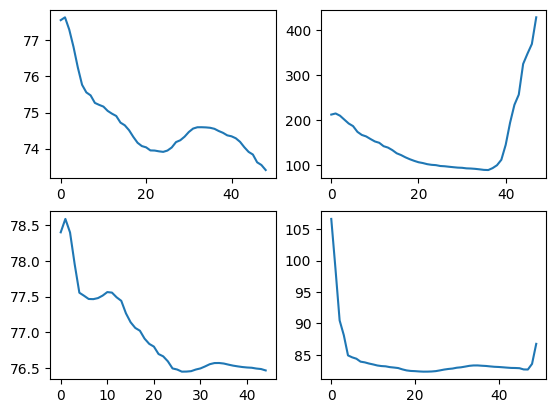
\includegraphics[width=0.5\textwidth]{sections/sensor_concepts/test_perch_profiles.png}
    \caption{Sample images from the proof of concept pipeline. The left images show 4 pairs of 
    parallel lines identified in figure \ref{fig:c1:testimg} (the parallel lines are drawn in green),
    as well as the perpendicular path traced for each pair of lines (the thicker line drawn in red).
    The right images show the depth profiles along the perpendicular path for each pair of lines.
    Note the high distortion around the edges of the target perch, particularly near the top end.
    The ideal depth profile for this perch would be a box function, where the high level indicates the
    distance to the perch and the width of the box corresponds to the width of the perch.
    }
    \label{fig:c1:depth_profiles}
\end{figure}

The depth images produces here have large amounts of noise and error, which interferes with identification of
suitable perches based on depth profiles. The errors in the depth image may be due to poor stereo calibration.
They may also be due to poor inpainting of missing regions. An attempt was made to implement the guided inpainting 
described by Gong et al. \cite{gong_guided_2013}, however so far implementing this algorithm has been unsuccesfull.




\subsubsection{Concept 2}

This concept is similar to concept 1, however it attempts to reduce weight and cost by estimating
a depth map from a single camera using optical flow and IMU measurements. This method would depend on 
the drone moving enough to measure optical flow, this motion could be artificially introduced to the 
position control algorithm, or could be naturally occurring corrections for wind or controller error.

Zingg et al. have successfully used optical flow for obstacle detection and avoidance, however their application
was primarily concerned with distances in the periphery of the cameras view. Due to only considering 
the drones speed in the cameras z-axis, their method lost accuracy in the center of the frame \cite{zingg_mav_2010}.
This application would require perch detection anywhere in the frame, and so will need to consider all velocity components
in estimating depth.

To estimate depth using all velocity coponents, the following method is used:

\begin{itemize}
    \item Between two images captured at $t_1$ and $t_2 = T_1 + \Delta t$, the drone has average velocity $\bar{v}$.
    \item A given point in the image appears to move from $\bar{r_1}$ to $\bar{r_2}$ between the two frames,
            due to the motion of the camera. The magnitude of both vectors is assumed to be similar, and 
            approximately equal to $D$, the distance to the object.
    \item The displacement of the drone between the two images is $\bar{d_1} = \bar{v} \Delta t$.
    \item The scene will appear to move the same distance in the opposite direction from the perspective 
            of an assumed stationary camera. This displacement is $\bar{d_2} = -\bar{d_1}$.
    \item Using Farneback optical flow, which provides dense estimates of pixel displacement $\bar{OF}$,
            a pixel coordinate $\bar{p_1}$ in the image at $$t_1$$ can be matched to another pixel $\bar{p_2}$
            at $t_2$ as $\bar{p_2} = \bar{p_1} + \bar{OF}$
    \item The angle between $\bar{p_1}$ and $\bar{p_2}$ is equal to the angle between $\bar{r_1}$ and $\bar{r_2}$,
            and can be found using the dot product of $\bar{p_1}$ and $\bar{p_2}$.
    \item Using the law of cosines and the assumption that $|\bar{r_1}| \approx |\bar{r_2}| \approx D$,
            $D$ can be estimated using equation \ref{eqn:dist_modified}
\end{itemize}

Note that in the process used by Zingg et al. \cite{zingg_mav_2010} a rotation is applied to the optical flow
vectors which removes optical flow caused by the rotation of the camera(as this optical flow is independent of
distance, and therefore provides no useful information). The same step is also applied to the optical flow vectors
used here, before estimating distance.

\begin{eqn}[H]
    \begin{equation}
        \begin{aligned}
            \label{eqn:dist_modified}
            cos(\theta) = \frac{\bar{p_1} \cdot \bar{p_2}}{|\bar{p_1}|  |\bar{p_2}|}
            \\
            D = \sqrt{\frac{(\Delta t |\bar{v}|)^2}{2(1 - cos(\theta))}}
        \end{aligned}
    \end{equation}
    Where:
    \begin{itemize}
        \item $\bar{v}$ is the average velocity over timestep $\Delta t$.
        \item $\bar{p_1}$ is a pixel coordinate in the first image.
        \item $\bar{p_2}$ is the pixel coordinate that optical flow identifies 
                as matched to the coordinate $\bar{p_1}$.
    \end{itemize}
\end{eqn}

\paragraph{Budget}

An IMU is included in the budget for this experimental project, however it would not need to be a part
of device if used on a real drone, as most drones already have an IMU built into their control system.

\begin{table}[ht]
    \centering
    \caption{Estimated budget for the optical flow sensing design.}
    \label{tab:flow}


    \begin{spreadtab}{{tabular}{|c|c|c|c||c|}}
        \hline
        @Item                       & @Supplier                                                                                                         & @Unit Cost (USD) & @Quantity & @Total Cost (USD) \\
        \hline
        @SMA Wire                   & @\href{https://www.kelloggsresearchlabs.com/product/round-wire/}{Kelloggs Research Labs}                          & 15.99 & 1 & [-1,0] * [-2,0] tag(start) \\
        @Mechanical Materials and Fabrication & @-                                                                                                      &     0 & 1 & [-1,0] * [-2,0] tag(pretax)\\
        @Tax                        & @- & sum(cell(start):cell(pretax)) * 0.07 & 1 & [-1,0] * [-2,0] tag(posttax) \\
        @Misc. Spares               & @- & sum(cell(start):cell(posttax)) * 0.2 & 1 & [-1,0] * [-2,0] tag(end) \\
        \hline
        \multicolumn{4}{|c||}{@Total} & sum(cell(start):cell(end)) \\
        \hline
    \end{spreadtab}
\end{table}

\paragraph{Evaluation}

There are two theoretical issues with this design. The first is that it assumes the scene in the camera to be stationary;
that the only source of optical flow is the motion of the drone. That assumption will not often hold when viewing a wind
blown branch or power line. The other issue is that the example use case in Zingg et al. \cite{zingg_mav_2010} is not 
computing a full depth image; it simply is estimating if objects are approaching closer on the left or right hand side
of the frame and generates a control signal to steer the opposite direction. The accuracy of this depth estimation is 
sufficient for steering down a straight hallway, but that does not mean it will produce a depth map sufficient to detect 
a straight line.

The modified depth estimation has been tested with one sample video from the Mid-Air dataset \cite{fonder_mid-air_2019}.
The velocity and pose ground truth data have been interpolated to the same sample rate as the video and depth frames.
Fig. \ref{fig:c2:depth} shows a sample frame from the ground truth data, 
and Fig. \ref{fig:c2:depth_est} shows an example depth estimate from this process.
The depth estimation process produces very large estimates in some locations,
which cause the displayed image to appear as all 0 to these large singularities
overshadowing other data in the image scaling. To ensure the image can be displayed with 
useful data, values in the estimated image with a depth of over 500m are set to \texttt{nan}.
Pixels set to \texttt{nan} appear white in the displayed image.

\begin{figure}[H]
    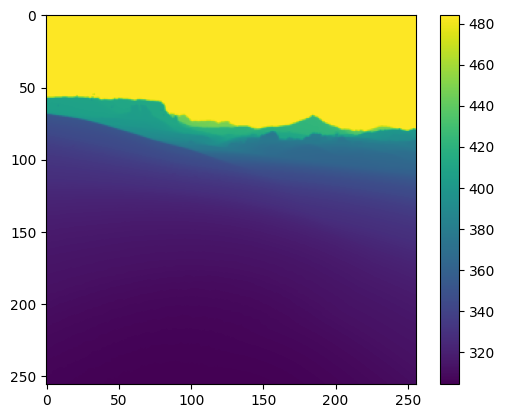
\includegraphics[width=\textwidth]{sections/sensor_concepts/ground_truth.png}
    \caption{Sample true depth image from the MidAir dataset. Depth values are in meters.
        Adapted from \cite{fonder_mid-air_2019}.}
    \label{fig:c2:depth}
\end{figure}

\begin{figure}[H]
    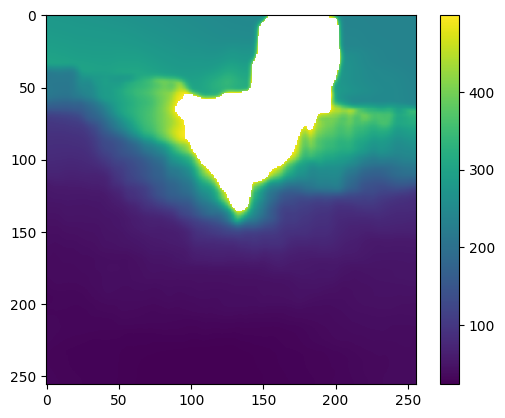
\includegraphics[width=\textwidth]{sections/sensor_concepts/estimate.png}
    \caption{Sample monocular depth estimation using the proposed method. Depth values are in meters.}
    \label{fig:c2:depth_est}
\end{figure}

\subsubsection{Concept 3}

This design would eliminate cameras entirely from the sensing design and use a simple time-of-flight
distance sensor mounted on a rotating servo, allowing it to sweep across a line above the drone to detect a perch.

\paragraph{Budget}

\begin{table}[ht]
    \centering
    \caption{Estimated budget for the lidar sensing design.}
    \label{tab:lidar}


    \begin{spreadtab}{{tabular}{|c|c|c|c||c|}}
        \hline
        @Item                       & @Supplier                                                                                                         & @Unit Cost (USD) & @Quantity & @Total Cost (USD) \\
        \hline
        @SMA Wire                   & @\href{https://www.kelloggsresearchlabs.com/product/round-wire/}{Kelloggs Research Labs}                          & 15.99 & 1 & [-1,0] * [-2,0] tag(start) \\
        @Mechanical Materials and Fabrication & @-                                                                                                      &     0 & 1 & [-1,0] * [-2,0] tag(pretax)\\
        @Tax                        & @- & sum(cell(start):cell(pretax)) * 0.07 & 1 & [-1,0] * [-2,0] tag(posttax) \\
        @Misc. Spares               & @- & sum(cell(start):cell(posttax)) * 0.2 & 1 & [-1,0] * [-2,0] tag(end) \\
        \hline
        \multicolumn{4}{|c||}{@Total} & sum(cell(start):cell(end)) \\
        \hline
    \end{spreadtab}
\end{table}

\paragraph{Evaluation}

This method would be computationally simpler than the camera based systems, though more mechanically
complex and possibly heavier. Additionally it would be unable to detect the orientation of a cylindrical 
perch, due to only measuring a cross section of the object.


\subsection{Concept Selection}

